\subsection{Exact old vision interfaces with selective current computation}
\label{app:vit_deployment}

We transferred the construction to ImageNet-pretrained ViT-B/32 on
CIFAR-100. The first ten transformer blocks form a shared frozen
prefix. The healthy two-block suffix produces the old representation
$h_0$ and its last MLP activation $u_0$. We fit a student fine-class
readout on their concatenation. Every old reader still receives
$h_0$. The student learns the current output of a saved teacher, and
a gate can send selected prefix tokens through that teacher's
updated two-block suffix.

The three teachers came from contrastive continuation, two-view
supervised continuation and doubled-epoch supervised continuation.
They used the same 20\% fitting-label budget. Each student received
both fixed views of the same 10,000 fitting images, using its own
teacher targets without further labels. We first fit an affine
residual with ridge coefficients $0.001,0.01,0.1,1$. The pilot retained
the contrastive-loss advantage but lost $0.76$--$1.04$ points of
joint-teacher accuracy. A nonlinear logit residual added 128 or
512 GELU units. We trained it for 30 epochs with normalized
centered MSE and unit-temperature KL, batch 256 and Adam at $0.001$.
The affine term stayed fixed after its ridge-$0.001$ fit. Width 128
lost $0.32$ points on the pilot, slightly beyond the $0.25$-point
retention margin; we kept this failed selection result.

For each student, the routing score is the gap between its two
largest logits. Cutoffs are quantiles of that score on clean fitting
images. We evaluated the fixed $10\%$, $25\%$ and $50\%$ quantiles.
The single-reference pilot selected $10\%$. Across twelve
training-only validation continuations, that point had an uncertain
retention interval. Final calibration averaged three continuations
within each of four fitted references and selected $25\%$, the
smallest point meeting the original gain and retention limits.
We fixed this rule before official-test predictions. Preparation of
healthy test features supplied no student or teacher accuracy for
selection. Teacher and student fitting, including the 128-unit
choice, used the training partition throughout.

\begin{proposition}[A retained interface and a selective current output]
\label{prop:selective_current}
Let $h_0(x)$ be the retained healthy representation, $C$ any fixed
consumer, $S$ a student classifier, $T$ its teacher and $r(x)\in\{0,1\}$
a routing rule. Define
\[
 F_r(x)=
 \begin{cases}
 T(x),&r(x)=1,\\
 S(x),&r(x)=0.
 \end{cases}
\]
Returning $C(h_0(x))$ preserves that consumer for every $x$ in real
arithmetic, independently of $S,T,r$. On any finite audit corpus,
for any assignment of task labels,
\[
 \left|\operatorname{err}(F_r)-\operatorname{err}(T)\right|
 \leq \frac{1}{n}\sum_{i=1}^{n}
     \mathbf 1\{r(x_i)=0,\ S(x_i)\ne T(x_i)\}.
\]
\end{proposition}
\begin{proof}
The old path computes the original composition. On routed inputs
the current output equals the teacher; on unrouted inputs, its error
indicator can differ only when student and teacher decisions differ.
Summing that pointwise inequality gives the bound.
\end{proof}

The gate uses confidence as in adaptive inference
\citep{bolukbasi2017adaptive}. Here, extra computation serves the new
output while the old interface always follows its retained path.
The proof concerns complete consumer functions, including their
normalization and thresholds. The current-task bound can be measured
without semantic labels on the audited inputs.

\begin{figure}[t]
\centering
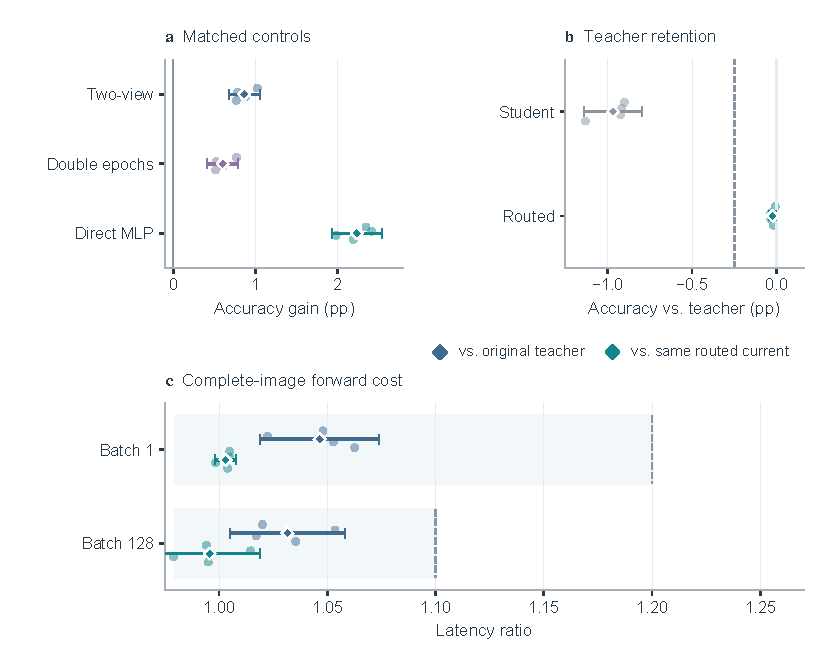
\includegraphics[width=\linewidth]{figures/fig_vit_deployment.pdf}
\caption{Official CIFAR-100 evaluation of the fixed visual program.
Small points are the four fitted-reference means, each averaging
three continuations; diamonds and bars show means and paired $95\%$
intervals. (a) Routed joint-student gains over three supervised controls.
(b) Accuracy change from the unrestricted joint teacher for the student,
the exact expectation of uniform random routing with equal calls, and
the fixed confidence route. The dashed line is the $-0.25$-point margin.
(c) Full-image CPU cost against the original teacher and the same
routed current function. Row-specific marks show the $1.20/1.10$
cost limits.}
\label{fig:vit_deployment_detail}
\end{figure}

On all 10,000 official test images, the routed joint program gains
$0.86 [0.68, 1.05]$ points over the routed two-view student and
$0.60 [0.41, 0.79]$ over the routed doubled-epoch student. Its change
from the unrestricted joint teacher is $-0.023 [-0.044, -0.003]$ points.
It uses the current teacher on $32.2\%$ of inputs.
The pure nonlinear student gains $0.52 [0.18, 0.87]$ and
$0.31 [0.06, 0.56]$ points, respectively, but loses
$-0.97 [-1.14, -0.79]$ points from its teacher. Thus the test distinguishes
a useful one-pass student from the point that also retains teacher
accuracy.

A direct supervised control uses the same retained features, 128-unit
head, fitting views, labels, 30 epochs and optimizer. Its affine
term can also learn. The routed joint program exceeds this control by
$2.23 [1.93, 2.54]$ points. The twelve programs use four historical fitted
references and the same TorchVision pretrained weights. The official
test images were reserved from every fit and model-selection phase;
intervals describe variation across the four reference means.

To separate routing quality from extra computation, we performed a
retrospective equal-call control on the saved predictions. For a uniform
subset of exactly $k$ of $n$ inputs, each teacher prediction is used with
probability $p=k/n$. Its expected accuracy is therefore
$(1-p)\operatorname{acc}(S)+p\operatorname{acc}(T)$, and its expected
teacher disagreement is $(1-p)D(S,T)$. We set $k$ to each fixed program's
actual call count. The confidence route exceeds this exact random
expectation by $0.63$ points $[0.51,0.75]$. It captures $99.33\%$
$[99.06,99.59]$ of student--teacher class differences. Remaining teacher
disagreement is $0.041\%$ $[0.023,0.058]$, versus $4.095\%$
$[3.848,4.343]$ under random routing. Thus the chosen inputs matter,
even at the same additional suffix-evaluation count. This comparison
uses already inspected test outputs; it introduces no new fitted policy
or independent confirmation. Call counts do not equate measured latency.

The old fine and coarse consumers each have a class rule and two fixed
confidence rules. Every audited rule agrees. The largest current-class
disagreement from the full joint teacher is $0.06\%$ across
the twelve programs, so their accuracy gaps on this corpus are bounded
by $0.06$ points for any labels
(Proposition~\ref{prop:selective_current}).

We measured complete FP32 image forwards with twelve physical CPU
cores on one NUMA node. A first traced implementation evaluated one
padded suffix item per batch. Its ratios were $1.162 [1.104, 1.220]$ at batch 1
and $1.047 [0.984, 1.110]$ at batch 128, missing the confidence-limit gates.
Scripted branches skip empty teacher sets, yielding
$1.046 [1.019, 1.074]\times$ and $1.032 [1.005, 1.058]\times$.
Batch-one blocks average 32 fixed images; batch 128 uses the first 128.
Nine alternating blocks yield one paired ratio per reference.
The implementation preserves all 120,000 current predictions,
720,000 old-rule decisions and 384 individual-input executions.
The archive retains the padded failure and excluded overlapping timing.
